% JuliaCon proceedings template
\documentclass{juliacon}
\setcounter{page}{1}

% You can use the command \mathlarger of the relsize package.
% It increases the size and it can be nested
\usepackage{amsmath}
\usepackage{relsize}

% You can use the package algoritmic for algorithms
\usepackage[lined,linesnumbered,ruled,vlined]{algorithm2e}
\usepackage{float}

\begin{document}

% **************GENERATED FILE, DO NOT EDIT**************

\title{Markov Chain-Monte Carlo Methods for\\ Linear Algebra using Julia v.1.0}

\author[1]{Oscar A. Esquivel-Flores}
\author[1]{Héctor Benítez-Pérez}
%\author[2]{3rd author}
\affil[1]{Universidad Nacional Autónoma de México, IIMAS-DISCA.}
%\affil[2]{National Lab}

\keywords{Julia, Monte Carlo Methods, Linear Algebra}



\maketitle

\begin{abstract}

A well known probabilistic method for solving systems of linear algebraic equations (SLAE) is Markov Chain-Monte Carlo (MCMC) method. Some works about this method have focused on estimating the solution vector, inverse matrix of the system and computing efficient preconditioner in order to obtain a good approximate solution. The iterative process, random sampling, compute a Markov Chain with appropriete length, compute the estimators of solutuion  represent an exhaustive computational effor for MCMC method as the size of SLAE increases. Some proposals to tackle the above are serial implementation using an efficient programming language and  parallel  implementation of MCMC on different parallel architecture.\verb Julia programming language has captured our attention since it has consolidated, relatively fast, as an excellent tool for scientific computation, therefore we have open a new route in our work by implementing the MCMC in \verb+ Julia v.1.0+ in order to accelerate the precision of the method without to paralelize it. This work presents our first iteration over MCMC using this alluring programming language.  

\headingtable

\end{abstract}

\section{Introduction}
Solving systems of linear algebraic equations (SLAE) in the form of $Ax = b$ or
inverting a real matrix $A$ is of unquestionable importance in many scientific fields. Iterative solvers are used widely to compute the solutions of these systems and such approaches are often the method of choice due to their predictability and reliability when considering accuracy and speed. They are, however, prohibitive for large-scale problems as they can be very time consuming to compute. These methods are dependent on the size of the matrix and so the computational effort grows with the problem size. The complexity of these methods is $O(kn^2)$ for dense matrices in the iterative case and $O(n^3)$ for direct methods with dense matrices while solving SLAE if common elimination or annihilation schemes (e.g. Gaussian elimination, Gauss-Jordan methods) are employed~\cite{golub1996matrix}. Therefore, these algorithms often rely on
preconditioners to speed up the computations and/or to ensure faster convergence.

Monte~Carlo (MC) methods on the other hand can quickly yield a rough estimate of the solution. This is done by performing random sampling of a certain variable whose mathematical expectation is the desired solution. For some problems an estimate is sufficient or even favourable, due to the accuracy of the underlying data. For example we would not need to process data with a higher precision than the one of the input data. In addition, Monte Carlo methods help to qualify the uncertainties while obtaining solution vector or performing matrix inversion. For example, Monte Carlo approaches enable to estimate the non-zero elements of the solution vector or inverse matrix with a given precision, and with certain probability.

Therefore, we concentrate on Monte~Carlo method that only require $O(NL)$ steps to find a estimate of vector solution. Here $N$ is the number of Markov chains and $L$ is an estimate of the chain length in the stochastic process. These computations are independent of the matrix size $n$ and also inherently parallel. Note that in order to find the inverse matrix or the full solution vector in the serial case, $O(nNL)$ steps are required. 

Depending on the method used to compute the vector solution or inverse matrix, the savings and end-results vary. Compute vector solution or inverse matrix of a very sparse system is quickly, but it is unlikey to improve the quality of the solution. On the other hand, compute the solution vector or inverse matrix of a dense system is computationally expensive and might be time or cost prohibitive. Therefore, finding a good solution for both problems that is computationally efficient, while still providing substantial improvement to the iterative solution process, is a worthwile research topic. 

The next section \ref{section_related_work} gives and overview of related work. Monte Carlo methods, and the specific matrix inversion algorithm that is discussed are presented in Section~\ref{section_algorithm}. Section~\ref{section_experiments} provides background information on the underlying computing systems and the experimental set ups. Results and findings from experiments with matrices of varying sizes and sparsity, as well as outcomes from running the SLAE solvers with  Monte Carlo inverse matrix are discussed in Section~\ref{section_evaluation}. The last Section~\ref{section_conclusion} consists of  the conclusion and  outlines the future work.

\section{Related Work}
\label{section_related_work}
Research efforts in the past have been directed towards optimizing the approach of computing the solution of SLAE through sparse approximate inverse matrix. 

The Monte Carlo code shown in this paper is part of a bigger family, it includes a serial algorithm for finding the vector solution of sparse systems of linear algebraic equations. The proposed Monte Carlo algorithm has been developed and enhanced upon in the last decades, and several key advances in serial and parallel Monte Carlo methods for solving such problems have been made~\cite{Alexandrov2005, alexandrov1999parallel, Branford2008grid, Dimov1998convergent, Dimov2007,
Fathi2002mixedmc}.

In the past there have been differing aproaches and advances towards a parallelisation of Monte Carlo methods using different kinds of programming languages in order to get a efficient vector solution and efficient matrix inversion used as preconditioner.

Several improvements of the Monte Carlo methods have been presented, some approaches use quasi-random sequences in order to  increase the rate of convergence of stochastic simulation algorithms~\cite{Atanassov2018, alexandrov2018}. Recently a new walk on equations Monte Carlo algorithm for solving SLAEs is proposed, this algorithm relies on a non-discounted  sum of an absorbed random walk~\cite{dimov2015}. 

Recently parallel approaches of MCMC method have been made using advanced accelerator architectures~\cite{lebedev2018}. 


\section{Monte~Carlo Approach}
\label{section_algorithm}

Monte~Carlo methods are probabilistic methods, that use random numbers to either simulate a stochastic behaviour or to estimate the solution of a problem. Method involves many independent samples used to estimate the solution, accuracy could be better when this sample increases, this consideration stress the computational effort. 

\subsection{General MCMC method for solving SLAE}
The following procedure has been presented by Fathi and Hassanzadeh in~\cite{Fathi-Vajargah2018}, they provide the basic background of the Monte Carlo Methods for solving SLAE and some modifications on the hybrid MC method to obtain accurate Matrix Inversion.

Assume that the System of Linear Algebraic Equations has the following form:
\begin{equation}
\label{slae-1}
Ax = b 
\end{equation}
where $A \in \mathbb{R}^{n \times n}$ is a nonsingular matrix and $x \in \mathbb{R}^n$ is a solution vector, $B \in \mathbb{R}^n$ is a known vector.

Consider the separation of matrix $A$ as $A =  M - N$ and subtitute in Equation (\ref{slae-1}, as shown in \cite{Fathi2002mixedmc} the system could be transformed in the following iterative scheme: 
\begin{equation}
\label{itsc-2}
x^{(k+1)} = Tx^{(k)}+f, k = 0,1,2,... 
\end{equation}
where $T = M^{-1}N$ and $f = M^{-1}b$.

The outcome of reducing the norm $\left \| T \right \| < 1$ (for a some matrix norm $\left \| \cdot \right \| < 1$) produces the convergence of iterative relation (\ref{itsc-2}) to exact solution of (\ref{slae-1}) regardless of the initial vector $x^0$ and thus reducing the number of Markov chains requiered to reach a given precision.

Assume that $\left \| T \right \| < 1$ and system is tranformed in (\ref{itsc-2}) consider a homogeneous discrete Markov chain $$\gamma : r_0 \rightarrow r_1 \rightarrow \dots r_k \rightarrow \cdots , $$ where $r_i\, i = 1,2,...,k$ belongs to the state space $R={1,2,...,n}$, which is built using random walks on the indices of $T$ in order to sample the solution of (\ref{slae-1}). 

Random walks are based on transition probabilities, wich requires the intital probability which make the initial probability vector $p \in \mathbb{R}^n$ (starting point of random walks) and transition probability matrix  $P \in \mathbb{R}^{n\times n}$ (transition from the current point to the next point) to satisfy the following conditions: 
\begin{equation}
\label{prob-3}
 \begin{array}{l}
 p_{ij} \geq 0, \quad \mathlarger{\sum}_{j=1}^{n} p_{i j}=1, \quad \text { if  } t_{ij} \neq 0 \quad \text { then  } p_{i j} \neq 0 \\ \\ p_i \geq 0, \quad \mathlarger{\sum}_{i=1}^{n} p_{i}=1, \quad \text { if  } h_{i} \neq 0 \quad \text { then } p_{i} \neq 0
 \end{array} 
\end{equation}

MCMC method is considered with uniform transition probability (UM) $P_{ij} = \frac{1}{n}$. Probability $P_{ij} = \frac{| T_{ij} |}{\sum_{j=1}^n | T_{ij} |}$ hs been used in Almost Optimal MCMC method (MAO) which satisfies transition conditions (\ref{prob-3}).

The distribution $p$ is acceptable for a given nonzero vector $h$, and that the distribution $P$ is acceptable for matrix $T$ \cite{branford2005}. The role of $h$ is restricted to the construction of the initial probability.

Fathi and Hassanzadeh~\cite{Fathi-Vajargah2018} define the following unbiased estimator for the stochastic trajectory $\gamma$:
\begin{equation}
\label{espx-4}
    X(\gamma) = \mathlarger \sum_{m = 0}^{\infty} W_mf_{r_m}
\end{equation}
where $W_m = W_{m-1}w_{r_{m-1}r_m}, w_{r_{m-1}r_m}=\frac{t_{r_{m-1}}r_m}{p_{r_{m-1}}r_m}$ and $W_0=\frac{h_{r_0}}{p_{r_0}}$ so that mathematical expectation of $X(\gamma)$ is the Euclidean inner product  $\left \langle h,x \right \rangle$, \textit{i.e.} $E[X_i(\gamma)]=x_i$ (see~\cite{dimov2015} and references therein).

Under condition $\left \| T \right \| < 1$ the corresponding Neumann series converges for any given $h$: 
\begin{equation}
 \label{newser-3}
  x = \sum_{k=0}^{\infty}T^kf 
\end{equation}
Thus to find an arbitrary component of the solution, for example the $i-th$ component of $x$, it should choose $h=e_i=(\underset{i}{\underbrace{0,...,1}},...,0)$ and $p_i=1$. They represent the single component of $x$ in the form:
\begin{equation}
 \label{sums-6}
 x_i = f_i + \mathlarger{\sum}_{m=1}^{\infty} \mathlarger{\sum}_{r_1 = 1}^{n} \mathlarger{\sum}_{r_2 = 1}^{n} \dots \mathlarger{\sum}_{r_m = 1}^{n} t_{ir_1} t_{r_1r_2} \dots t_{r_{m-1}r_m}f_{r_m} \quad ,
\end{equation}
it can be proved that mathematical expectation of $X_i(\gamma)=\sum_{m=0}^{\infty}W_mf_{r_m}(h=e_i, p_i=1)$ is the $i-$th component of the solution, i.e., $E[X_i(\gamma)]=x_i$~\cite{dimov2015}.

Using the following notation for the partial sum $X_i(\gamma_k)=\sum_{m=0}^{k}W_mf_{r_m}$ on finite Markov chain $\gamma : r_0 \rightarrow r_1 \rightarrow \dots r_k$ whose mathematical expectation tends to $x_i$ by choosing $k$ large enough. This approximation leads to the systematic error.

\subsection{Systematic and Statistical Errors}

An stopping criterion for the random walk to create the Markov chain $\gamma_k$ is given by \textit{systematic error} $\left | W_k \right| < \epsilon$
where $\epsilon > 0$ is the given parameter. An upper bound for length of Markov chain $\gamma_k$ can be computed sustituting the value of $\left | W_k \right| < \epsilon$, thus:  
\begin{equation}
 \begin{array}{ll}
 \left|W_{k}\right|=| \frac{t_{r_{0} r_{1}} t_{r_{1} r_{2}} \dots t_{r_{k-1} r_{k}}}{p_{r_{0} r_{1}} p_{r_{1} r_{2}} \cdots p_{r_{k-1} r_{k}}} | &  \le \frac{t_{r_{0} r_{1}} t_{r_{1} r_{2}} \dots t_{r_{k-1} r_{k}}} {\frac{t_{r_{0} r_{1}}}{\left \| T \right \|} \frac{t_{r_{1} r_{2}}}{\left \| T \right \|} \dots \frac{t_{r_{k-1} r_{k}}}{\left \| T \right \|}} \\
 & < {\left \| T \right \|}^k
 \end{array}
\end{equation}
Accordingly $k < \frac{log(\epsilon)}{log \left \| T \right \|}$.

The fact of $\left \| T \right \| \le 1$ reduces the length of Markov chain and convergence speed of the MCMC method increases. Simulating $N$ independent sample paths of the Markovian Chain $${r_0}^{(s)} \rightarrow {r_1}^{(s)} \rightarrow \cdots \rightarrow {r_k}^{(s)}, \quad  s = 1,2, \cdots ,N $$ and consider the sample mean of $X_i(\gamma_k^{(s)})$ to estimate the real mean $E[X_i(\gamma_k)]$ \textit{i.e.} $\overline{X}_i(\gamma_k)= \frac{1}{N}\sum_{s=1}^N X_i(\gamma_k^{(s)}) \approx x_i $.\\

The \textit{probable error} of the method is defined as $r_N = 0.6745\sqrt{\frac{var(X)}{N}}$ where:
$$P\{ \left|\overline{X} - E\left[ X \right] \right| < r_N \} \approx 1/2 \approx P\{ \left|\overline{X}-E\left[X\right] \right| > r_N \}$$ if it has $N$ independent realizations of random variable $X_i(\gamma_k)$, with mathematical expectation $E[X]= E\left[X_i\left(\gamma_k\right)\right]$ and average $\overline{X} = \overline{X}_i(\gamma_k)$ \cite{branford2005}. Probable error is employed to estimate the statistical error.
The \textit{statistical error} is expressed as:$\left|\overline{X}_i\left(\gamma_k \right)-E\left[X_i\left(\gamma_k\right)\right]\right|<\delta$, where $\delta$ is the given parameter. Using the precision the precision $r_N \le \delta$ and employing the upper bound for $var(X_i(\gamma))$, it results: 
\begin{equation}
 \label{vln-7}
 N \ge \frac{(0.6745)^2}{\delta^2} \frac{{\left \| f \right \|}^2}{(1-\left \| f \right \|)^2}
\end{equation}

Algorithm~\ref{algo:mcmc1} presents the MCMC method~\cite{Fathi-Vajargah2018}.

%----------------------- Algorithm 1 ---------------------------------
%\twocolumn[
%\begin{@twocolumnfalse}

%\begin{center}
%\scalebox{1.0}{
%\begin{minipage}{0.7\linewidth}
 \begin{algorithm}[!h] % H = forzar esta posición
  \DontPrintSemicolon
  %\caption{MCMC}
  \label{algo:mcmc1}
  \SetAlgoLined
  \KwData{$T,\,  f, \, \epsilon, \delta $}
  \KwResult{$X_i(\gamma_k)$}
  \LinesNumbered
  \SetAlgoVlined
  Compute  $ N = \left [ \frac{(0.6745)^2}{\delta^2} \frac{{\left \| f \right \|}^2}{(1-\left \| T \right \|)^2} \right ] + 1 $ \;
  Compute $P$ based on the type of probability transition matrix\;
  \For{$i=1$ to $n$}{
     \For{$s=1$ to N}{
       Set $W_0=1, k=0, point = i, X_i^{(s)}= W_0f_i$\;
       \While{$|W_k| \ge \epsilon $}{
         Generate an r.v. $nextpoint$, distributed on $i-th$ row of matrix $P$ as:\;
         Set $nextpoint = 1$, $u=rand$ \;
           \While{$u > P_{ponint,nextpoint}$}{
             $nextpoint = nexpoint + 1$
             } %\EWhile
         Set $k = k +1$\;
         \If{$t_{point,nextpoint} \ne 0$}{
            Compute \;
            $W_k = W_{k-1}\frac{t_{point,nextpoint}}{P_{point,nextpoint}}$, \;
            $X_i^{(s)} = X_i^{(s)}+W_k f_{nextpoint}$       
           }
        Set $point = nextpoint$
        }
      }
      Compute $X_i(\gamma_k) = \frac{1}{N} \mathlarger{\sum}_{s=1}^N {X_i^{(s)}}$
  }
  %\label{algo:mcmc1a}
  \caption{MCMC Algoritm for solving SLAE} 
 \end{algorithm}
%\end{minipage}
%} % scalebox
%\end{center}
%\end{@twocolumnfalse}
%]   %end twocolumn
%-----------------------------------------------------------------

\subsection{Markov Chain-Monte Carlo method in Julia}

Implementation of the MCMC method in Julia is transparent and very similar to the code presented in  (\ref{algo:mcmc1}) in practice, the main packages requiered were: \verb Statistics, \verb LinearAlgebra, and \verb SparseArrays . 

\begin{lstlisting}[language = Julia]
# Compute T and f

M = diagm(0 => diag(A));
N = M-A;
T = inv(M) * N;
f = inv(M) * b;
    
# Compute P and p probability matrices

nT, mT = size(T);
S = fill(0, nT);
[S[i] += 1 for i in 1:nT, j in 1:mT if T[i,j] != 0];
P = fill(0., nT, mT); 
[P[i,j]= 1/S[i] for i in 1:nT, j in 1:mT if T[i,j] != 0 ];

# Compute number of chains
N = floor((0.6745/δ)^2*((norm(f)^2)/(1-norm(T))^2)) + 1 # Se calcula N

# Compute MCMC method
Xs = fill(0., mT)
for i in 1:mT
  W_0 = 1
  for s in 1:N
     W = W_0; point = i; X = W_0 * f[i]
     while abs(W) >= ϵ
        nextpoint  = 1
        u = rand()
        while u >= sum(P[point, 1:nextpoint])
           nextpoint = nextpoint + 1
        end
        if T[point, nextpoint] != 0 
           W_new = W *(T[point, nextpoint]/P[point, nextpoint])
           X = X + W_new * f[nextpoint]
        end
        point = nextpoint
        W = W_new
     end
     Xs[i] += X
  end
end
x_mc = Xs/N;

\end{lstlisting}


\section{Experiments}
\label{section_experiments}

In this paper we focus on the precision of the algorithm that works on sparse matrices.  We are interested in testing how varying the precision, e.g. the systematic error $\delta$ and the probabilistic error $\epsilon$,  influences the quality of the Monte Carlo approximate solution. Tests were made in an x86 CPU architecture consist in a Intel Core i7 vPro CPU, 8Gb RAM.

In order to studying the Marko Chain-Monte Carlo method for solving systems of linear algebraic equations it is relevant not only to take abstract matrices but matrices which represent a concrete problem to solve. This section presents some tests about a matrix that represents the physical behavior of the temperature in a bidimiensional square domain which experiences diffusion. Mathematically, the system $Ax=b$ is defined by the following partial equation $$\frac{\partial(\rho C_vT) }{\partial t} = \nabla \cdot (\kappa \nabla T)$$ where $\rho$, $t$, $C_v$, $T$ and $\kappa$ represent density, time, specific heat, temperature and thermal conductivity respectively. It's worth to mention that test matrix was obtained with finite volume method; dimesions of test matrix $A$ are of $120 \times 120$ and vector $b$ is a column vector of size $120$. Figure\ref{fig:testmtx} shows the sparsity pattern of the test matrix.

\begin{figure}[h]
 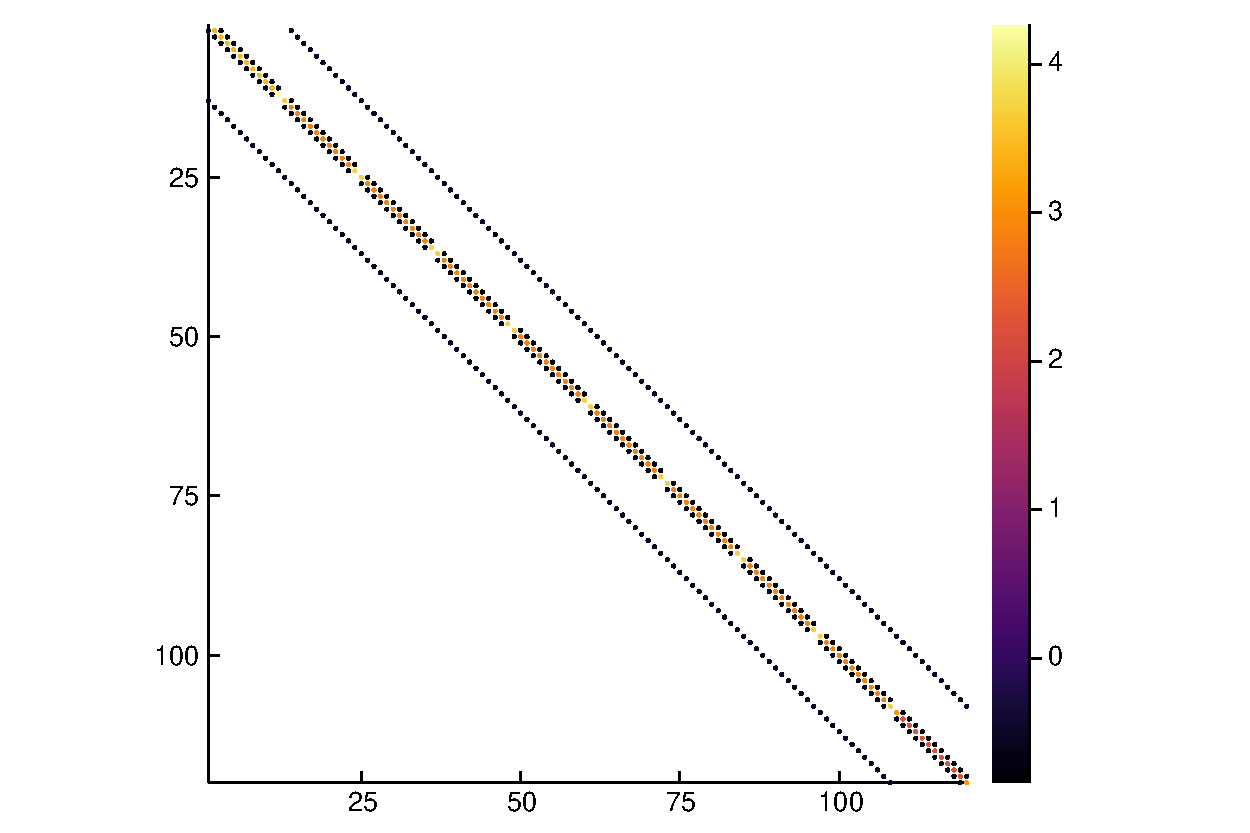
\includegraphics[height=2.5in, width=3.8in]{testmtx}
 \caption{Sparsity pattern and entrie's values of test matrix}
 \label{fig:testmtx}
\end{figure} 

Matrix $A$ is used as input to the algorithm \ref{algo:mcmc1} to compute the accuracy of the approximate solutiton variying the $\epsilon$ and $\delta$ parameters.

In order to show the output of \verb BenchmarkTools  macro some experiments was developed using values of $\epsilon = 0.1$ and $\delta=0.1$ 
\begin{verbatim}
BenchmarkTools.Trial: 
  memory estimate:  375.43 MiB
  allocs estimate:  977796
  --------------
  minimum time:     178.927 ms (21.18% GC)
  median time:      192.165 ms (20.70% GC)
  mean time:        198.074 ms (22.14% GC)
  maximum time:     280.477 ms (47.87% GC)
  --------------
  samples:          26
  evals/sample:     1
\end{verbatim}

Table \ref{table:etimnorm} shows the compute times and the 2-norms of $\left \|b - A\hat{x} \right \|_2$ for different values of parameters.

\begin{table}[!h]
\tabcolsep15pt
\tbl{Number of Markov Chains $N$, $\left \|b - A\hat{x} \right \|_2$ and execution time for different values of $\epsilon$ and $\delta$}{
\scalebox{0.90}{
\begin{tabular}{lllll}\hline
%\multicolumn{5}{c}{\textbf{Matrix properties}}                                                                                                                      \\ %\hline
$\epsilon$    & $\delta$ & $N$ &  $\left \| \cdot \right \|_2$ & time(s) \\ \hline %& \multicolumn{1}{c}{Description}                                                                                        \\ \hline
0.1 & 0.1 & 4 & 6.729 & 0.188\\
0.1 & 0.05 & 14 & 5.174 & 0.553 \\
0.1 & 0.01 & 330 & 1.05 & 12.07\\
0.1 & 0.005 & 1319 & 0.56 & 47.62\\
0.1 & 0.001 & 32961 & 0.22 &1203.2\\ \hline
0.05 & 0.1 & 4 & 6.69 & 0.263\\
0.05 & 0.05 & 14 & 5.67 & 0.662 \\
0.05 & 0.01 & 330 & 0.94 & 14.168 \\
0.05 & 0.005 & 1319 & 0.50 & 56.96 \\
0.05 & 0.001 & 32961 & 0.154 & 1435.9 \\ \hline
0.01 & 0.1 & 4 & 6.65 & 0.292 \\
0.01 & 0.05 & 14 & 3.60 & 0.839 \\
0.01 & 0.01 & 330 & 1.06 & 19.12\\
0.01 & 0.005 & 1319 & 0.55 & 76.25\\
0.01 & 0.001 & 32961 & 0.154 & 2142.0 \\ \hline
0.005 & 0.1 & 4 & 6.92 & 0.323 \\
0.005 & 0.05 & 14 & 3.21 & 0.948 \\
0.005 & 0.01 & 330 & 1.05 & 20.79 \\
0.005 & 0.005 & 1319 & 0.69 & 84.62 \\
0.005 & 0.001 & 32961 & 0.11 & 2149.7\\ \hline
0.001 & 0.1 & 4 & 6.36 & 0.394 \\
0.001 & 0.05 & 14 & 3.05 & 1.14\\
0.001 & 0.01 & 330 & 1.00 & 25.60 \\
0.001 & 0.005 & 1319 & 0.62 & 102.25 \\
0.001 & 0.001 & 32961 & 0.18 & 2611.7\\ \hline

\end{tabular}}
}
\label{table:etimnorm}
\end{table}

Previous results shows the influence of the parameter associated with the error statistic $\delta$ as the one that most strongly influences the accuracy and time of execution of the implementation. The proposed case of temperature diffusion over a domain it was observed that the accuracy of the method improves in each temporary step although the results suggest that this precision is limited.

Figure \ref{fig:time} shows the impact of parameters $\epsilon $ and $\delta$ on executime time. Results show that parameter $\delta$ increses the execution time when it takes values less than or equal to $0.005$ because this parameter defines the number of markov chains that will be constructed to estimate each input of the solution vector. Figure \ref{fig:norm} shows the impact of parameters $\epsilon $ and $\delta$ on accuray of the method. Results show there is not any impact of parameter $\epsilon$ on accuracy, however, the accuracy increases ($\left \|b - A\hat{x} \right \|_2$ decreses) when the $\delta$ parameter is decreasing and the number of markov chains increases.

Finally, figure shows the relationship between the precision of MCMC method and execution time. It is unquestionable that accuracy depends on the number of Markov chains $N$ built for estimating each entry of the solution vector, which sacrifices the efficiency in orden to achieve some precision.  


\begin{figure}[h!]
 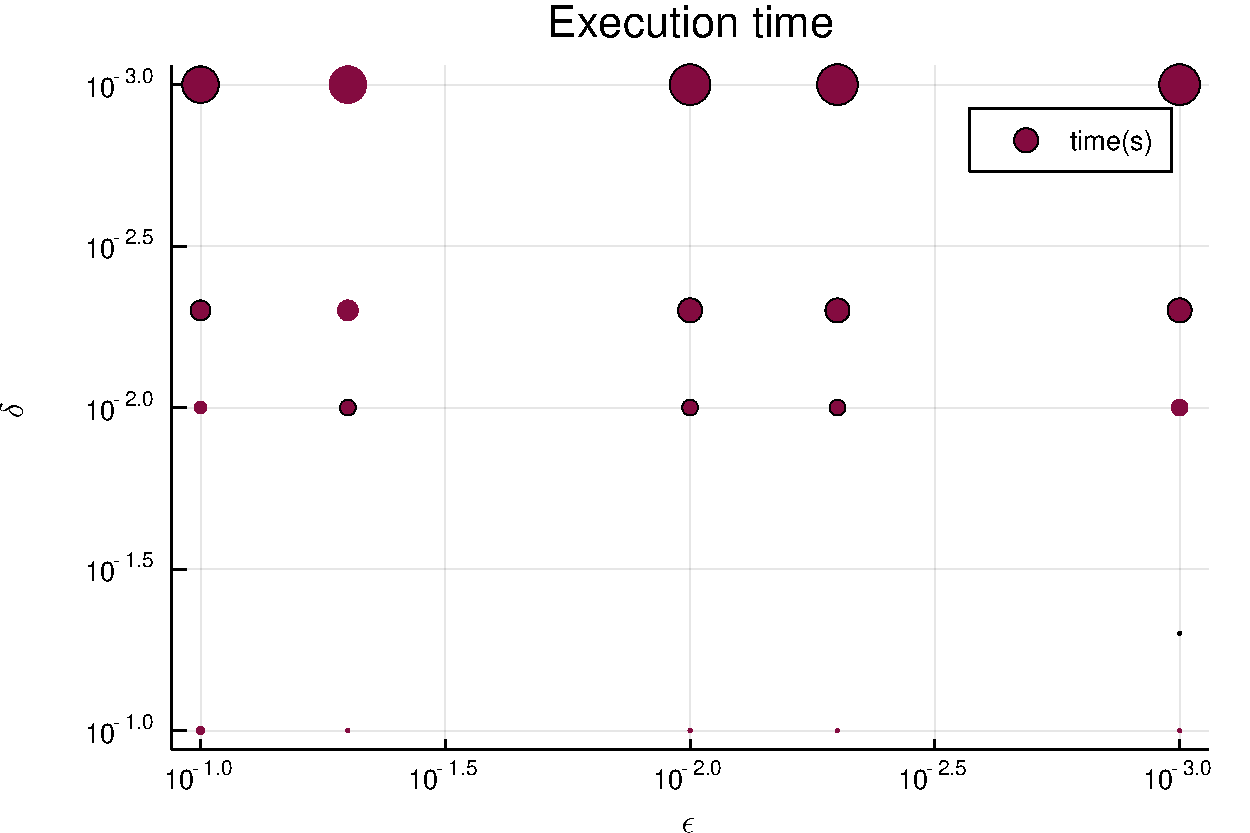
\includegraphics[height=2.0in, width=3.3in]{exectime}
 \caption{MCMC execution times for different values of $\epsilon$ and $\delta$ parameters}
 \label{fig:time}
\end{figure}

\begin{figure}[h!]
 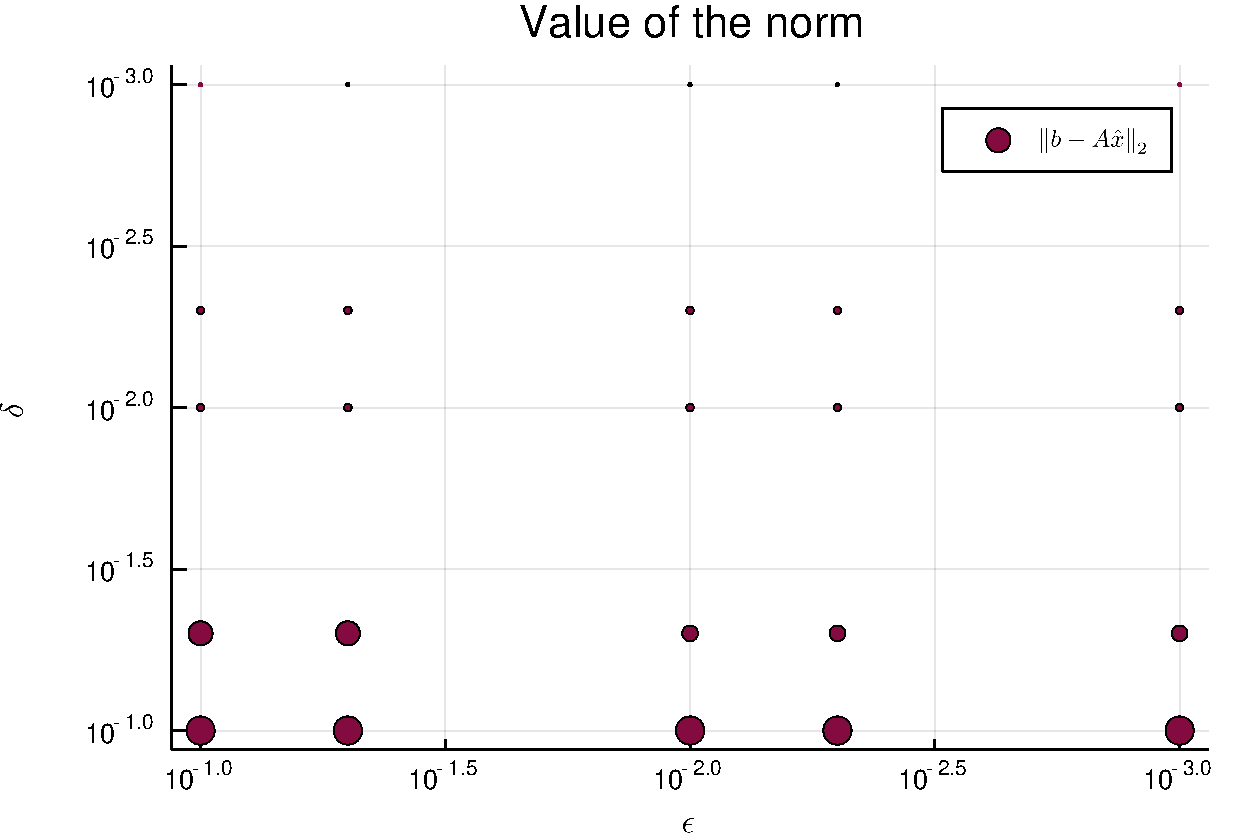
\includegraphics[height=2.0in, width=3.3in]{norm.pdf}
 \caption{MCMC accuracy for different values of $\epsilon$ and $\delta$ parameters}
 \label{fig:norm}
\end{figure} 

\begin{figure}[h!]
 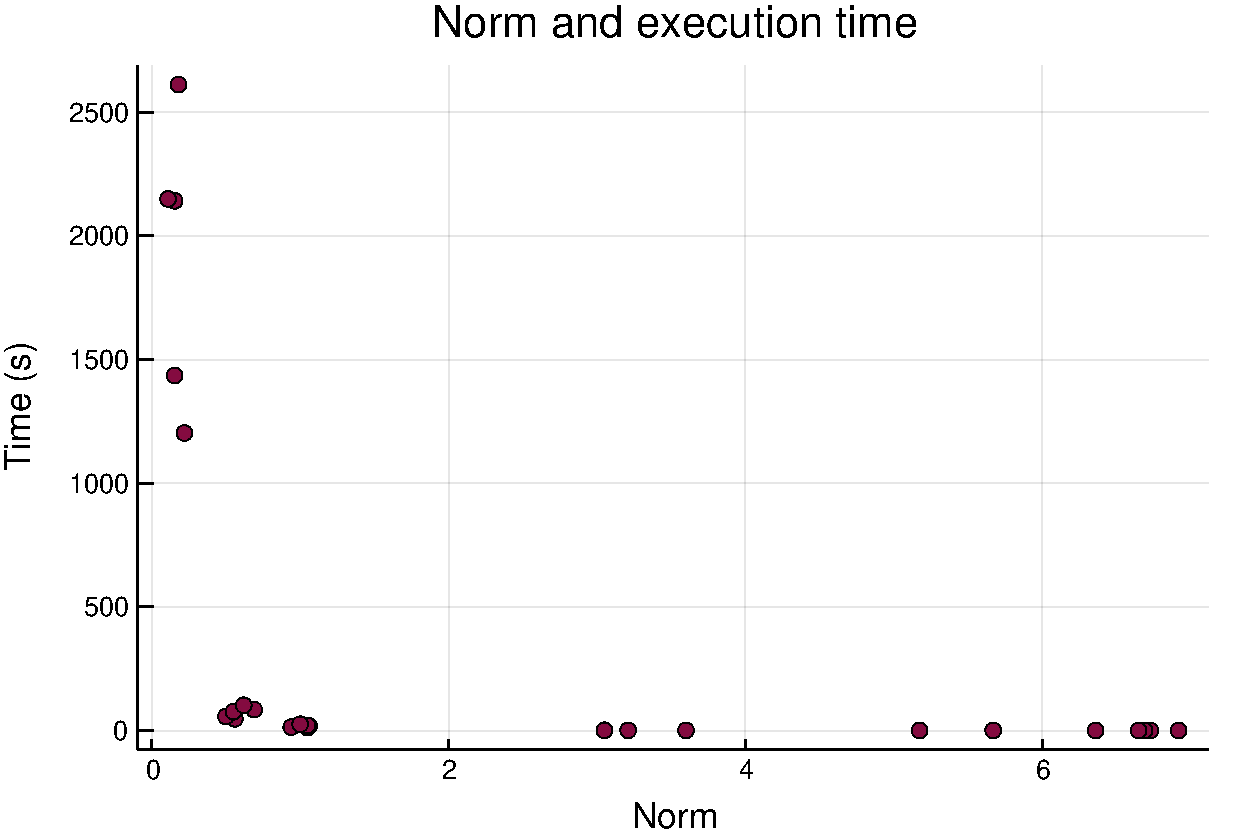
\includegraphics[height=2.0in, width=3.3in]{normtime.pdf}
 \caption{Relationship}
 \label{fig:normtime}
\end{figure} 

\section{Evaluation}
\label{section_evaluation}

Further experiments were carried out to investigate how varying the precision parameters impacts on the approximate Monte Carlo delivering  an efficient solution to SLAEs.
 
Consider the computational experiments on selected matrices given in table~\ref{table:etimnorm}. First, it is evident that increasing the precision $\epsilon$ does not lead to any significant  increase of the execution time of Monte Carlo algorithm. Therefore in many cases it is beneficial to obtain the Monte Carlo approximate solution using very rough precision, and also keeping the systematic and probable errors to be of the same magnitude, so that to minimize the execution time of the algorithm.

Second, it should be noted that increasing the precision $\delta$ does lead to significant  increase of the execution time and precision of MCMC algorithm. This shows a susbstantial gain, it is possible to obtain the MCMC approximate solution of SLAE much more accurate by sacrificing the number of iterations to achieve this precision.

\section{Conclusions and Future Work}
\label{section_conclusion}

A Markov Chain-Monte Carlo method based approximate solution and the corresponding algorithm for solving SLAEs have been presented as an alternative strategy. MCMC algorithm has been implemented in Julia v.1.0 which enables increasing the time in analysis. Several adavantages by implementing the MCMC method in Julia v.1.0. are worth to note. Transparent syntax, very fast even in a single multicore processor. Packages as \verb LinearAlgebra, \verb Statistics, and \verb SparseArray were very useful in order to compute norms, random variables, and optimize calculation over \verb+sparse arrays+.

The study of the parameters that define the accuracy of the method allows us to know its limitations and make decisions about the level of precision desired, which can be low and be fine-tuned by means of other iterative techniques.

As future work we can mention tha
Ssome works have proposed MCMC algorithm is well suited for calculating preconditioners for SLAE solvers \cite{StrassburgAlexandrov2014, AlexandrovEsquivel2015} using classes of matrices such as  non-diagonally dominant and  non-symmetric matrices; particularly taken matrices from different sets  obtained from \textit{Suite Sparse Matrix Collection} \footnote{https://sparse.tamu.edu/} (this repository actually merge two previous collections -The Matrix Market~\cite{boisvert1996matrix} and The University of Florida Sparse Matrix Collection~\cite{davis2011university}). \verb MatrixDepot  and \verb SparseArrays  Julia packages are efficient tools in order to get and easily manipulate benchmark sparse matrices, future work deals with manipulate test matrices using this packages.

Finally, MCMC method is highly parallelizable. The support for NVIDIA GPUs to the Julia programming language \cite{besard2017} promises to be an excellent help to program GPUs devices in order to increase the accuracy of the method and the speed of execution.

\section*{Acknowledgements}
We would like to thank to José Antonio Borrás Gutiérrez (post graduate student in UNAM) by sharing the test matrices, we hope Antonio evolves for Python to Julia very soon.  


%---------------------------------------------------------

% **************GENERATED FILE, DO NOT EDIT**************

\bibliographystyle{juliacon}
\bibliography{ref.bib}


\end{document}
